%\section{Retrospective}

%¿cómo estabamos al principio?

When this project started we had access to numerous image analysis and visualization tools (see chapter \ref{chap_related}). However these tools are designed to work with specific data types, and thus integrating data from different sources required significant work. Additionally most of these tools have a step learning curve, which is appropriate for image experts but leaves them out of reach for users from other domains. Experts from domains different to radiology required to go trough the radiologist or an engineer in order to access image data. Moreover clinical data was always on separate files, which meant it was necessary to switch application in order to get context information about a subject. Typical image based analysis involved extracting scalar features from images, which were later added to a table, and then analyzed in statistical software together with clinical data. This analysis was usually completed using tables. Generating plots required additional steps and was done only for communication purposes. The risk of this approach was that outliers or pathological data could go undetected. 

The current project was conceived to address these issues. Using the proposed tools it is possible to access image data instantaneously,  for image experts, but also for experts from different domains. In addition these images are showed with context and they can be linked to additional information of a given subject. Scalar features extracted from image data can be visually analyzed together with clinical data. In this way outliers immediately draw attention, can be identified and analyzed in more detail. Experts from all domains can access spatial data, think about it, and propose analyzes. In contrast, before most analyzes involving spatial data were proposed by image experts and limited to existing tools. These analyzes will still need the help of image experts for performing the required calculations and interpreting the results; and possibly from engineers if new tools need to be developed. By making data available to the whole team, this way of thinking becomes possible.    

% ¿Como ha anvanzado nuestra comprension del problema?
% ¿de los datos?
% ¿de los usuarios?
% ¿de las necesidades?
In order to better assess the benefits and limitations of the proposed approach, we conducted several interviews with potential users, applied surveys, and did a group session. These activities and their results will be explained in this chapter. Additionally it will be explained how the model from Chapter \ref{chap_model} can be used to generate applications requested by users.	

% ¿qué problemas nuevos han surgido?
% ¿qué oportunidades?
% ¿hacia dónde vamos?

\section{Work with potential users}

An important part of the requirements analysis for the project was carried out at CHUL in Quebec, Canada. Specifically, the Axes Neurosciences group was a significant contributor. This group researches the functioning of the nervous system in healthy and pathilogical conditions. One of the methods used is performing experiments on large numbers of participants. During these experiments they collect data from each participant using neuro-psychological tests, measurements of muscle strength and movement, neuro-image and TMS tests. 

% Knwoldedge depends on the hypotheses, and the hypotheses on the technology available for testing the questions raised. 
 
%Description of the lab, software used, prism, aabel, statistica, labchart, excel, 
% Cyril's team
% Cyril's TMS publication
%The tms applications

One of the interests of the group was analyzing relationships between TMS outcomes and white matter structure as portrayed by DWI and tractography. The particular TMS experiment tested the connections from the primary motor cortex to the hand muscles, and between the motor cortices at both hemipsheres (see \autocite{schneider_cerebral_2012}). For this purpose an specific application was designed, it showed the values of the TMS outcome together with visualizations of the relevant fiber bundles. Screen-shots of the finished application can be seen on figures \ref{fig_tms_1} and \ref{fig_tms_2}). 

\begin{figure}
	\centering
		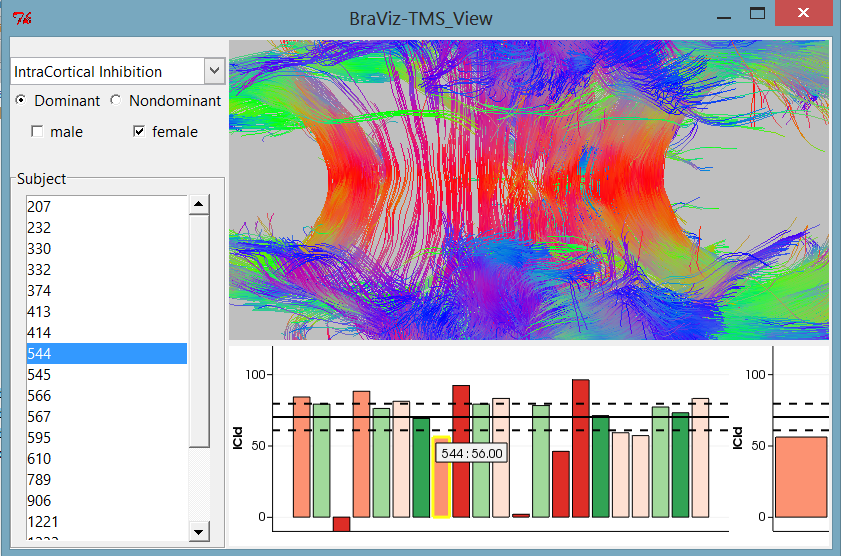
\includegraphics[width=0.90\textwidth]{figures/analysis/tms_view_early}
	\caption{An early version of the TMS viewer application.}
	\label{fig_tms_view_early}
\end{figure}

Figure \ref{fig_tms_view_early} shows an earlier version of the application. In the top left side it had a combo-box for selecting one of the different outcomes. The radio buttons below allowed the researcher to choose between the metrics for the dominant or non-dominant side. Finally there was a list of subjects which could be filtered to show only males, only females or both. At the top right there was a 3D viewer which would display a relevant fiber bundle related to the current outcome. Specifically for intra-cortical measures it would show the motor fibers for the corresponding hemisphere (as in figure \ref{fig_tms_1}) while the corpus callosum would appear for Inter-hemispheric measures.
Below there was a bar plot showing the values of the current outcome for the current subject, together with a large display of this value on the right. The solid and dotted lines in the plot correspond to the mean and the interval within one standard deviation; these statistics are calculated considering only the subjects in the control group. Bars inside this interval are colored green while those outside are colored in red.
This layout was first designed on paper with one of the group researchers. 

The user could move trough subjects either by selecting a code on the list or by clicking on one of the bars. The bar at the right would change to the new value, using a transition to accentuate the difference. The image will also change to that of the new subject. This simple tool allows the researcher to navigate between the TMS-outcomes while looking at the underlying white matter structure. 

\begin{figure}
	\centering
		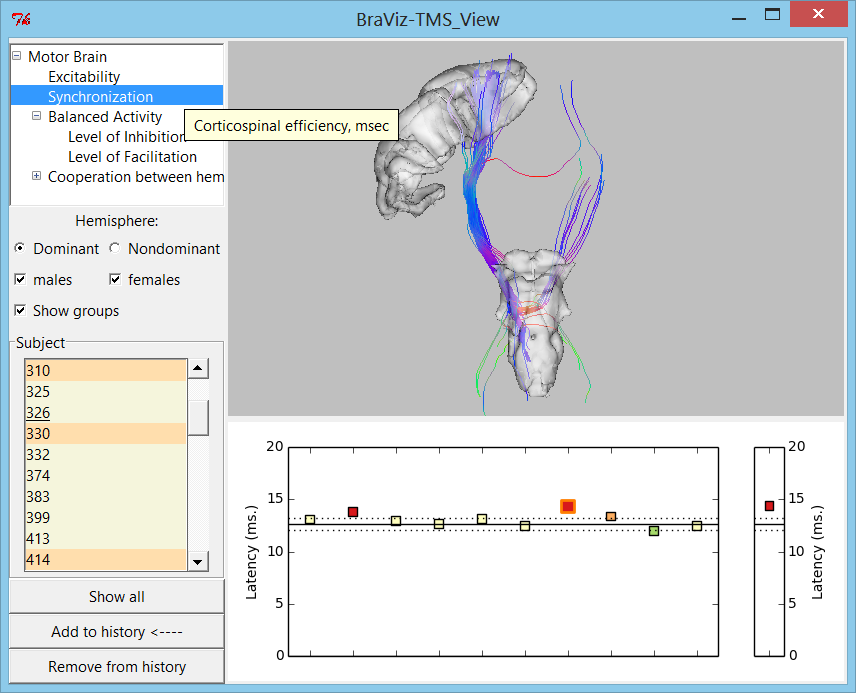
\includegraphics[width=0.90\textwidth]{figures/analysis/tms_view_motor}
	\caption{A second version of the TMS-viewer application}
	\label{fig_tms_view_second}
\end{figure}

Figure \ref{fig_tms_view_second} shows a posterior version of this tool. After receiving feedback from the group, several improvements were made:
\begin{itemize}
	\item TMS outcomes are now organized in a tree, and more descriptive names are used. The purpose is to provide meaning to experts who have limited experience with TMS. Additionally tooltips were added in order to provide additional information on each metric.
	\item The underlying study involved three groups: kangaroo mother care, incubator and control. For some analysis it is convenient to be blind about these groups, but some other times it is beneficial to have this information. Now there is an option to show the different groups in the list of subjects by using different background colors.
	\item The axes in the plot are more clearly labeled and measurement units are shown. 
	\item For some outcomes a higher value is better, while for some others a lower value is better. Now values of the second type are showed using squares instead of bars.
	\item Colors in the main plot were redefined. Now red can be read as \emph{worst than controls}, yellow as \emph{similar to controls} and green as \emph{better than controls}.
	\item The main plot can show the complete sample or only some interesting subjects. The user may add or remove subjects to this sub-sample using the buttons below the subject list.
\end{itemize}

Another round of feedback produced the version shown in figure \ref{fig_tms_2}. This version included additional information in the 3D viewer in order to help users interpret it. The other major feature was showing grouped data in the main plot for the three groups in the study.

This tool allowed experts to .................\footnote{Help Cyril}.

% Veronique Manip
% finding correlations

% Anna Belle Manip

% Hugo Manip
% 

% Alyssa

KMC
	Marin
	Rejean
	Nathalie

% Video Conference from Iowa

% Ste Irenne

% lock patient

\section{Interest Surveys}
NIDCAP
Guttman's lab

\section{Group Test}

Ana Maria

\section{Building Applications}

Consequence of the model
Reusable components
Process, stages
metrics: time, lines of code
Other developers: David, Yoyis


\section{Discussion}

What features are the most useful?
What is feasible now that wasn't at the start?
What features are missing?
What limitations have come to light?

Can these techniques be used on other domains?



